\begin{figure}[ht]
    \centering
    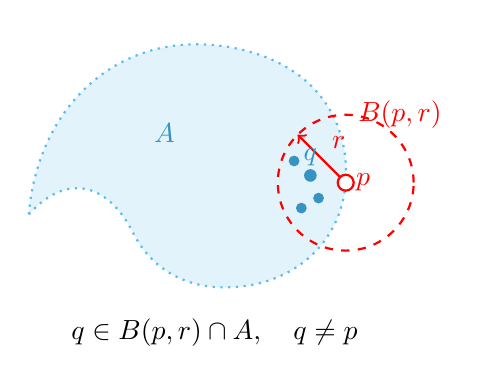
\begin{tikzpicture}[scale=1.15]
        % Conjunto A: uma região ameboide, preenchida sem fronteira desenhada.
        \path[fill=Cerulean!12]
            (-2.15,-0.15)
            .. controls (-2.05,1.05) and (-1.15,1.9) .. (0.05,1.7)
            .. controls (0.95,1.55) and (1.4,0.95) .. (1.35,0.2)
            .. controls (1.3,-0.45) and (0.8,-0.9) .. (0.15,-0.95)
            .. controls (-0.4,-1.0) and (-0.8,-0.75) .. (-1.0,-0.35)
            .. controls (-1.25,0.15) and (-1.7,0.35) .. (-2.15,-0.15)
            -- cycle;
        \draw[Cerulean!70, thick, dotted]
            (-2.15,-0.15)
            .. controls (-2.05,1.05) and (-1.15,1.9) .. (0.05,1.7)
            .. controls (0.95,1.55) and (1.4,0.95) .. (1.35,0.2)
            .. controls (1.3,-0.45) and (0.8,-0.9) .. (0.15,-0.95)
            .. controls (-0.4,-1.0) and (-0.8,-0.75) .. (-1.0,-0.35)
            .. controls (-1.25,0.15) and (-1.7,0.35) .. (-2.15,-0.15)
            -- cycle;

        % Ponto de fronteira e uma bola centrada nele.
        \coordinate (p) at (1.35,0.2);
        \draw[Red, thick, dashed] (p) circle (0.75);
        \draw[Red, thick, ->] (p) -- ++(135:0.75)
            node[midway, above right] {$r$};

        % Pontos de A dentro de B(p,r), diferentes de p.
        \filldraw[Cerulean!80!black] (0.96,0.28) circle (1.8pt) node[above] {$q$};
        \filldraw[Cerulean!80!black] (1.05,0.03) circle (1.5pt);
        \filldraw[Cerulean!80!black] (0.78,0.44) circle (1.5pt);
        \filldraw[Cerulean!80!black] (0.86,-0.08) circle (1.5pt);

        % O ponto p esta na fronteira da regiao.
        \draw[Red, thick, fill=white] (p) circle (2.5pt) node[right] {$p$};

        \node[Cerulean!80!black] at (-0.65,0.75) {$A$};
        \node[Red] at (1.95,0.95) {$B(p,r)$};
        \node at (-0.1,-1.45) {$q\in B(p,r)\cap A,\quad q\neq p$};
    \end{tikzpicture}
    \caption{Ilustração de um ponto de acumulação de um conjunto.}
\end{figure}
